\subsection{Resistance measurement}

\subsubsection{Idea}
\label{sec:method_resistance_idea}
With the overall feature idea being auto-range, the resistance measurement is no exception. We knew we needed more than one voltage divider, meaning more than one voltage divider with a known resistance of R1. See Figure \ref{fig:vol_div}. This means there needed to be a solution to be able to switch between these known resistors since the optimal configuration is to have the highest V$_{\text{CC}}$ possible, for better accuracy. This can be done by either removing the V$_{\text{CC}}$ for the resistors not being used, or removing the ground plane.
In this case, we opted for removing V$_{\text{CC}}$, since we wanted to do this with transistors. We chose MOSFET specifically, since they have a very low impedance when saturated, compared to the average BJT. And since the voltage across the unknown resistor can vary between 0V to 5V, thus the Source-pin, the N-channel variation is not optimal, whereas the P-channel is well suited since the Source-pin is always the same. Hence, we opted for five different values, since that can cover a large enough resistance spectrum for our purpose. This also implies that we need five GPIO-pins, other than the analogue-pin, which we only have a limited supply of. But it is needed. For the schematic used, see section \ref{sec:appendix}, the full schematic, block 8. We opted for the P-channel MOSFET \textit{IRLML6401TRPBF}, since it proved to have a saturation impedance, R$_{\text{DS(ON)}}$, of only 0.05$\Omega$, limiting the parasitic resistance in our measurement of the known- and unknown resistor.

\begin{figure}[h]
    \centering
    \frame{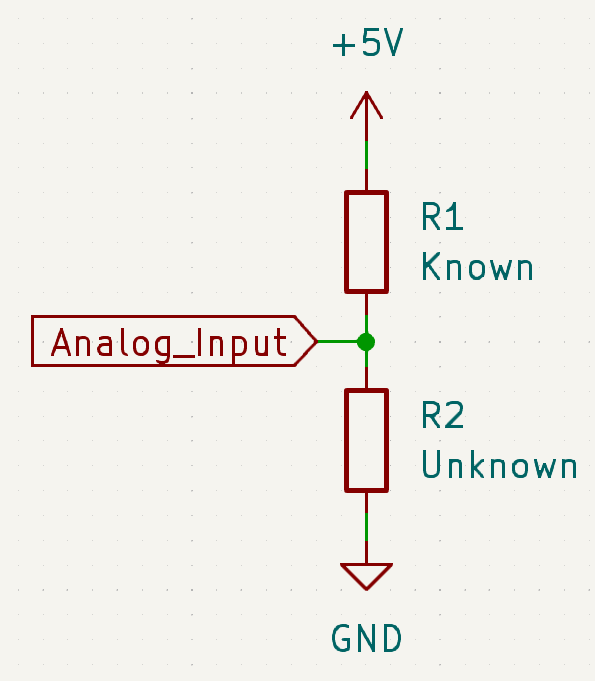
\includegraphics[scale=0.25]{images/Vol_div.png}}
    \caption{Voltage Divider setup}
    \label{fig:vol_div}
\end{figure}

\subsubsection{Code implementation}
\label{sec:method_resistance_code}
The data sampling and evaluation are done using two nested for-loops and a switch statement. The first loop iterates through as many times as it is declared beforehand using a constant. This loop is used for averaging out the final value. The second, inner for-loop does the data collection. The data is stored in an array, whose elements correspond to the measured values at the different resistance ranges. Using the function called \textit{setResistancePin}, the 5 control pins of the PMOS transistors are switched so that only one is active at any given time (the selected pin will be LOW, while the other pins HIGH). After the correct range has been selected using this method, the value measured by the ADC of the MCU is stored at the particular index of the array. There is a small delay of approximately 4 milliseconds between the measurements to let the voltage settle at the input pin. To get the range that is closest to 2.5V (half of the V$_{CC}$), the function \textit{getClosestToHalf} is used. This function iterates through the array of measured values and updates the correct index to be used by checking the size of the difference between the measured value and 512 (i.e. half of the maximum resolution of the built-in ADC, 10 bits - 1023 is the maximum value). After the correct index to be used is found, the values for the variables used in the final calculation are chosen in a switch statement. The value of the unknown resistance is found by the following formula:
\vspace{1cm}\[R_X=\frac{M*R_N}{2^A-1-M}\]
where: \[R_X , R_N , M , A\] are the unknown resistance value, known resistance value (selected range), the measured digital value and the resolution of the ADC, respectively. After the loops have finished, the result is averaged out. Before displaying the final value, a function called \textit{checkDisconnectedRes} is used to check whether there is an actual resistor connected to the input terminals or not. This function iterates through the array of measured values, checking whether the values are below a certain threshold value. If all the values at the specific ranges are below this threshold value, that means that there is nothing connected to the input terminals, thus nothing is displayed. Otherwise, the calculated resistance value and the selected range are displayed on the LCD screen. With this method, we can measure resistances from 0 $\Omega$ up to around 3 M$\Omega$ with adequate precision.

